\section{The \texorpdfstring{$q$}{q}-intersection determinant}\label{sec:qdet}
\begin{proof}[Proof of Theorem~\ref{thm:intersection-real}]
Let $\C$ be an essential real affine hyperplane arrangement with normal crossings.  By Theorem~\ref{thm:Lam-real},
\[
 \det\bigl((V_b^{-1})^{\cB}\bigr)
 =\frac{\displaystyle\prod_{F\in\cL_0\setminus\{E\}}
          (1-b_{E\setminus F}^2)^{w_F}}
        {\displaystyle\prod_{F\in\cL\setminus(\cL_0\cup\{\varnothing\})}
          (1-b_F^2)^{w_F}}.
\]

By Proposition~\ref{prop:normal-crossing-ranks}
and Lemma~\ref{lem:free-coextension},
the flats avoiding $0$ contribute only when they are singletons,
and the proper flats containing $0$ are $F=K\cup\{0\}$ for
$K\in\cL(M_0)\setminus\{E_0\}$. Put
\[
 \lambda_K=w_{K\cup\{0\}}
       =\beta(M_{0,K})\mup((M_0^K)^*).
\]
Specializing $b_i$ to $q$, for all $i\in E_0$, in the expression above gives
\[
 \det\bigl((V_q^{-1})^{\cB}\bigr)
 =\frac{\displaystyle\prod_{K\in\cL(M_0)\setminus\{E_0\}}
          (1-q^{2|E_0\setminus K|})^{\lambda_K}}
        {(1-q^2)^{\sum_{i\in E_0}w_{\{i\}}}}.
\]
The inverse-matrix identity of Corollary~\ref{thm:varinv} and
$|\cB|=\beta(M)$ therefore give
\[
 \det S_q
 =(1-q^2)^{r\beta(M)-\sum_{i\in E_0}w_{\{i\}}}
   \prod_{K\in\cL(M_0)\setminus\{E_0\}}
      (1-q^{2|E_0\setminus K|})^{\lambda_K}.
\]
Corollary~\ref{cor:degree} identifies the exponent outside the product
with $-\sum_K\lambda_K$. Hence
\[
 \det S_q
 =\prod_{K\in\cL(M_0)\setminus\{E_0\}}
    \left(\frac{1-q^{2|E_0\setminus K|}}{1-q^2}\right)^{\lambda_K}.
\]
If $K$ is not cyclic, $M_0^K$ has a coloop, so its dual has a loop
and $\mup((M_0^K)^*)=0$. The product reduces to
\eqref{eq:Sq-determinant}.
\end{proof}

The same calculation, using the oriented-matroid form of
Corollary~\ref{thm:varinv} and Lemma~\ref{lem:free-coextension},
proves the following reduction independently of realizability.

\begin{corollary}\label{cor:conjecture-reduction}
For a normal crossing affine oriented matroid, the conjectural determinant
formula \eqref{eq:Lam-determinant} implies \eqref{eq:Sq-determinant}.
\end{corollary}

\begin{example}\label{ex:four-lines}
Consider the two normal crossing arrangements $\C$ and $\C'$ below,
each consisting of four lines with $H_1\parallel H_2$. Put
$E_0=\{1,2,3,4\}$ and order their bounded chambers as
$\cB=(P_1,P_2)$ and $\cB'=(P'_1,P'_2)$, respectively.

\begin{center}
 \begin{minipage}{0.46\textwidth}
  \centering
  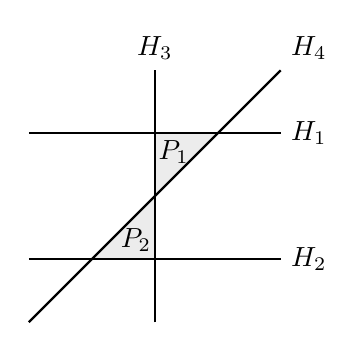
\begin{tikzpicture}[scale=0.8]
   \fill[gray!15] (0,0) -- (0,1) -- (1,1) -- cycle;
   \fill[gray!15] (0,0) -- (0,-1) -- (-1,-1) -- cycle;
   \draw[thick] (-2,1) -- (2,1) node[right] {$H_1$};
   \draw[thick] (-2,-1) -- (2,-1) node[right] {$H_2$};
   \draw[thick] (0,-2) -- (0,2) node[above] {$H_3$};
   \draw[thick] (-2,-2) -- (2,2) node[above right] {$H_4$};
   \node at (0.3,0.7) {$P_1$};
   \node at (-0.3,-0.7) {$P_2$};
  \end{tikzpicture}
  \par\smallskip
  $\C$
 \end{minipage}\hfill
 \begin{minipage}{0.46\textwidth}
  \centering
  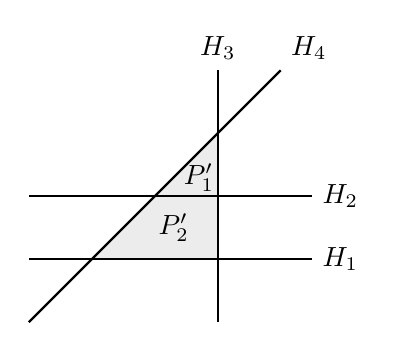
\begin{tikzpicture}[scale=0.8]
   \fill[gray!15] (0,0) -- (0,-1) -- (-1,-1) -- cycle;
   \fill[gray!15] (0,-1) -- (0,-2) -- (-2,-2) -- (-1,-1) -- cycle;
   \draw[thick] (-3,-2) -- (1.5,-2) node[right] {$H_1$};
   \draw[thick] (-3,-1) -- (1.5,-1) node[right] {$H_2$};
   \draw[thick] (0,-3) -- (0,1) node[above] {$H_3$};
   \draw[thick] (-3,-3) -- (1,1) node[above right] {$H_4$};
   \node at (-0.3,-0.7) {$P'_1$};
   \node at (-0.7,-1.5) {$P'_2$};
  \end{tikzpicture}
  \par\smallskip
  $\C'$
 \end{minipage}
\end{center}

In $\C$, the two bounded chambers are triangles whose closures meet
at a vertex. In $\C'$, they are a triangle and a quadrilateral whose
closures share an edge. Corollary~\ref{cor:multivariate-inverse} gives
\[
 \begin{aligned}
 \bigl(V_b(\C)^{-1}\bigr)^{\cB}
 ={}&(1-b_3^2)^{-1}(1-b_4^2)^{-1}\\
 &{}\cdot
 \begin{pmatrix}
  (1-b_{\{1,3,4\}}^2)(1-b_1^2)^{-1}&b_3b_4\\
  b_3b_4&(1-b_{\{2,3,4\}}^2)(1-b_2^2)^{-1}
 \end{pmatrix}
 \end{aligned}
\]
and
\[
 \begin{aligned}
 \bigl(V_b(\C')^{-1}\bigr)^{\cB'}
 ={}&(1-b_2^2)^{-1}(1-b_3^2)^{-1}(1-b_4^2)^{-1}\\
 &{}\cdot
 \begin{pmatrix}
  1-b_{\{2,3,4\}}^2&-b_2(1-b_{\{3,4\}}^2)\\
  -b_2(1-b_{\{3,4\}}^2)&
  (1-b_{\{1,2\}}^2)(1-b_{\{3,4\}}^2)(1-b_1^2)^{-1}
 \end{pmatrix}.
 \end{aligned}
\]
Both determinants are
\[
 \frac{(1-b_{E_0}^2)(1-b_{\{3,4\}}^2)}
 {(1-b_1^2)(1-b_2^2)(1-b_3^2)^2(1-b_4^2)^2}.
\]
This agrees with Theorem~\ref{thm:Lam-real}. For both arrangements,
the nonzero weights of proper nonempty flats of $M$ are
\[
 w_{\{0\}}=w_{\{0,1,2\}}=w_{\{1\}}=w_{\{2\}}=1,
 \qquad w_{\{3\}}=w_{\{4\}}=2.
\]

Setting $b_i=q$ and multiplying by $(1-q^2)^2$ gives
\[
 S_q(\C)=
 \begin{pmatrix}
  1+q^2+q^4&q^2\\
  q^2&1+q^2+q^4
 \end{pmatrix},\qquad
 S_q(\C')=
 \begin{pmatrix}
  1+q^2+q^4&-q(1+q^2)\\
  -q(1+q^2)&(1+q^2)^2
 \end{pmatrix}.
\]
Thus
\[
 \det S_q(\C)=\det S_q(\C')
 =(1+q^2)^2(1+q^4)=\qint{2}\,\qint{4}.
\]
The two factors correspond to the proper cyclic flats
$\{1,2\}$ and $\varnothing$ of $M_0$, each with exponent one in
Theorem~\ref{thm:intersection-real}.
\end{example}
